\chapter{A Companhia Aérea}
\label{chapter:Companhia Aérea}
A companhia aérea alvo deste trabalho é a Air Astana, tendo sido fundada no final de 2001, teve o seu voo inaugural a 15 de maio de 2002 e é constituída por dois acionistas, o Governo da República do Cazaquistão e a BAE Systems PLC do Reino Unido.
A sua inauguração contou com a presença dos dois, sendo o governo representado pelo na altura Presidente Nursultan Nazarbayev e a BAE Systems PLC por Sir Richard Evans.
O site da companhia pode ser acedido neste \href{https://airastana.com/global/en-us}{link}~\cite{link1}.\\
\indent As rotas que a companhia possui atualmente estão representadas no mapa que se segue:

\begin{figure}[h]
        \centering
        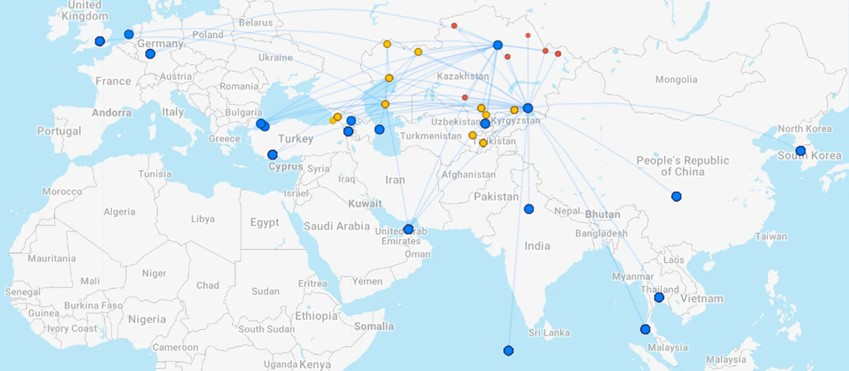
\includegraphics[width=1\textwidth]{imgs/Figura1}
        \caption{Mapa de rotas da Air Astana retirado de FlightConnections.com\label{fig:imagem1}}
\end{figure}

\noindent\underline{\textbf{Observações:}}\\
\begin{itemize}
\item Todos os pontos representados no mapa são destinos onde a Air Astana opera, por sua vez as rotas da
companhia são representadas pelas arestas.
\item A cor e o tamanho dos diferentes pontos assinalados no mapa é para serem ignorados, pois apenas
representam um número de voos diretos que os destinos recebem, no geral, de todas as companhias aéreas 
que tem rotas diretas para aquele mesmo destino. \href{https://www.flightconnections.com}{$($Fonte: site onde o mapa foi retirado$)$}~\cite{link2}

\item Um mapa de rotas, utilizamos como base este mapa interativo genérico de um site de terceiros, com o
propósito de mostrar as rotas, quando se aplicam certos filtros de pesquisa.
\item Para aceder ao site com o mapa acima apresentado, basta aceder \href{https://www.flightconnections.com/route-map-air-astana-kc}{aqui}~\cite{link3}.
\end{itemize}
\clearpage
\section{DESTINOS DA COMPANHIA PARA REPRESENTAR NO GRAFO}
Para futuros cálculos e representações do grafo relacionado, vamos enumerar os destinos:\\

\begin{figure}[h]
    \centering
    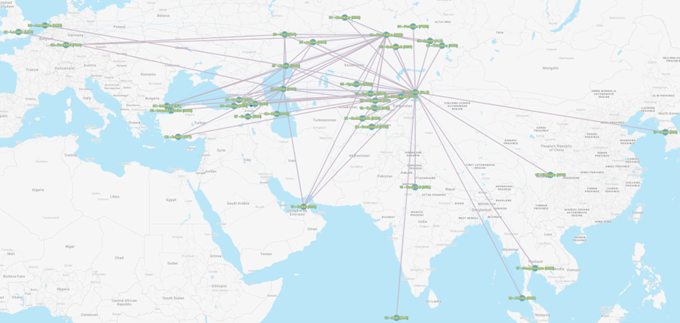
\includegraphics[width=1\textwidth]{imgs/Figura2}
    \caption{Mapa de rotas de voo da Air Astana com destinos nomeados.\label{fig:imagem2}}
\end{figure}


\begin{center}
\begin{tabular}{ l l }
        01 - Londres (LHR) & 19 - Seoul (ICN)\\
        02 - Amsterdão (AMS) & 20 - Duchambé (DYU)\\
        03 - Frankfurt (FRA) & 21 - Samarcanda (SKD)\\
        04 - Istambul (IST) &  22 - Turkistan (HSA)\\
        05 - Istambul Sabiha (SAW) & 23 - Shymkent (CIT)\\
        06 - Antália (AYT) & 24 - Bisqueque (FRU)\\
        07 - Erevan (EVN) & 25 - aqtöbe (AKX)\\
        08 - Tbilisi (TBS) & 26 - Oral (URA)\\
        09 - Baku (GYD) & 27 - Atyrau (GUW)\\
        10 - Dubai (DXB) & 28 - Aktau (SCO)\\
        11 - Nova Deli (DEL) & 29 - Kutaisi (KUT)\\
        12 - Tashkent (TAS) &  30 - Batumi (BUS)\\
        13 - Almaty (ALA) & 31 - Kostanay (KSN)\\
        14 - Nur-Sultan (NQZ) &  32 - Qyzylorda (KZO)\\
        15 - Malé (MLE) & 33 - Qarağandı (KGF)\\
        16 - Phuket (HKT) & 34 - Pavlodar (PWQ)\\
        17 - Banguecoque (BKK) & 35 - Semei (PLX)\\
        18 - Chengdu (CTU) & 36 - Öskemen (UKK)\\
\end{tabular}
\end{center}
